\documentclass[preview]{standalone}
\usepackage{tikz}
\begin{document}
%\begin{figure}
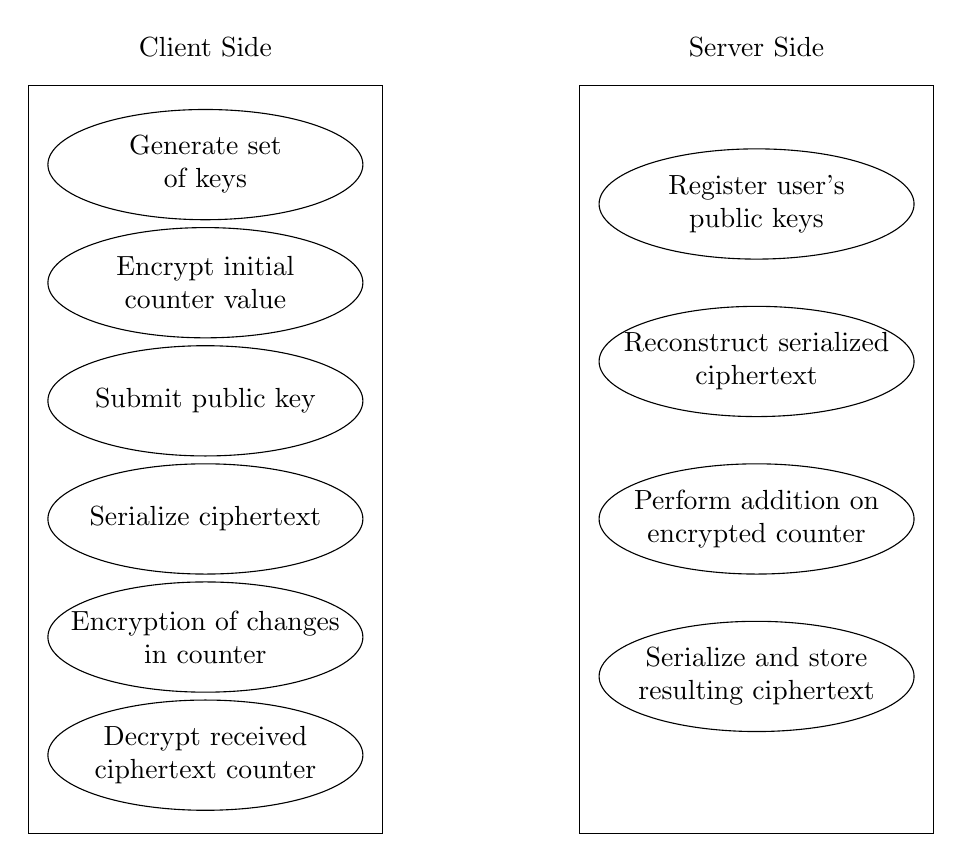
\begin{tikzpicture}
    %client
    \node[align=center] at (2.25, 10) {Client Side};
    \draw [black] (0,0) rectangle (4.5,9.5);
    \draw (2.25, 8.5) ellipse (2cm and 0.70cm);
    \node[align=center] at (2.25, 8.5) %
         {Generate set \\ of keys};
    \draw (2.25, 7) ellipse (2cm and 0.70cm);
    \node[align=center] at (2.25, 7) %
         {Encrypt initial \\ counter value};
    \draw (2.25, 5.5) ellipse (2cm and 0.70cm);
    \node[align=center] at (2.25, 5.5) %
         {Submit public key};
    \draw (2.25, 4) ellipse (2cm and 0.70cm);
    \node[align=center] at (2.25, 4) %
         {Serialize ciphertext};
    \draw (2.25, 2.5) ellipse (2cm and 0.70cm);
    \node[align=center] at (2.25, 2.5) %
         {Encryption of changes\\in counter};
    \draw (2.25, 1) ellipse (2cm and 0.70cm);
    \node[align=center] at (2.25, 1) %
         {Decrypt received\\ciphertext counter};
    %server
    \node[align=center] at (9.25, 10) {Server Side};
    \draw [black] (7,0) rectangle (11.5,9.5);

    \draw (9.25, 8) ellipse (2cm and 0.70cm);
    \node[align=center] at (9.25, 8) %
         {Register user's\\public keys};
    \draw (9.25, 6) ellipse (2cm and 0.70cm);
    \node[align=center] at (9.25, 6) %
         {Reconstruct serialized\\ciphertext};
    \draw (9.25, 4) ellipse (2cm and 0.70cm);
    \node[align=center] at (9.25, 4) %
         {Perform addition on\\encrypted counter};
    \draw (9.25, 2) ellipse (2cm and 0.70cm);
    \node[align=center] at (9.25, 2) %
         {Serialize and store\\resulting ciphertext};         
\end{tikzpicture}
%\caption{Architecture breakdown into client and server.}
%\end{figure}
\end{document}
